\documentclass[10pt,journal,compsoc]{IEEEtran}
\usepackage[utf8]{inputenc}
\usepackage[T1]{fontenc}
\usepackage{graphicx}
\usepackage{amsmath}
\usepackage{amsfonts}
\usepackage{amssymb}
\usepackage{booktabs}
\usepackage{hyperref}
\usepackage{cite}
\usepackage{float}
\usepackage{array}
\usepackage{multirow}
\usepackage{color}
\usepackage{xcolor}
\usepackage{listings}
\usepackage{url}

\definecolor{dkgreen}{rgb}{0,0.6,0}
\definecolor{gray}{rgb}{0.5,0.5,0.5}
\definecolor{mauve}{rgb}{0.58,0,0.82}

\lstset{frame=tb,
  language=Python,
  aboveskip=3mm,
  belowskip=3mm,
  showstringspaces=false,
  columns=flexible,
  basicstyle={\small\ttfamily},
  numbers=none,
  keywordstyle=\color{blue},
  commentstyle=\color{dkgreen},
  stringstyle=\color{mauve},
  breaklines=true,
  breakatwhitespace=true,
  tabsize=3
}

\begin{document}

\title{Koşullu Çekişmeli Üretici Ağlar ve MONAI UNet ile Bilgisayar Destekli Meme Tümörü Segmentasyonu\\
\small{(Enhanced Generative Adversarial Networks and MONAI UNet for Computer-Aided Breast Tumor Segmentation in MRI)}}

\author{Yasir~Ömer~Alparslan\\
Danışman: Prof.~Dr.~Osman~Özkaraca\\
Yapay Zeka Anabilim Dalı, Fen Bilimleri Enstitüsü\\
Muğla Sıtkı Koçman Üniversitesi, Muğla, Türkiye\\
\textit{E-posta: yasir.alparslan@ogr.mu.edu.tr}}

\markboth{Yüksek Lisans Araştırma Raporu -- Muğla Sıtkı Koçman Üniversitesi, 2026}%
{Alparslan: Koşullu GAN ve MONAI UNet ile MRG Meme Tümörü Segmentasyonu}

\IEEEtitleabstractindextext{%
\begin{abstract}
Yapay görme tabanlı medikal görüntü segmentasyonunda, temel alınan modellerin yapısal ve geometrik kararsızlıklarını gidermek kritik bir öneme sahiptir. Bu çalışmada, literatürdeki öncü BTS-GAN mimarisi \cite{haq2022bts} sistematik bir analize tabi tutulmuş; veri senkronizasyonu ile gradyan sönümlenmesi problemlerini çözen, üretime hazır bir derin öğrenme hattı geliştirilmiştir. Orijinal BTS-GAN modeli RIDER veri kümesi üzerinde Paralel Dilate Konvolüsyon (PDC) modülü kullanan özelleştirilmiş bir yapıya dayanırken, önerilen kararlı mimaride üreteç (generator) bileşeni medikal standartlara uygun MONAI UNet \cite{monai} ile değiştirilmiş, ayırt edici (discriminator) olarak ise PatchGAN tercih edilmiştir. Deneysel çalışmalar, BreastDM veri kümesi \cite{breastdm2023} kullanılarak NVIDIA RTX PRO 6000 Blackwell mimarisinin yüksek hesaplama gücü eşliğinde yürütülmüştür. Beş bileşenli hibrit bir kayıp fonksiyonu topluluğu (BCE, Dice, Focal, L1 ve GAN Kaybı) ve geometrik olarak senkronize edilmiş veri artırma stratejileriyle eğitilen modelimiz; test veri setinde 0.811 Zar Katsayısı (DSC), 0.738 Kesişim-Birleşim (IOU) ve 0.886 Keskinlik (Precision) değerlerine ulaşmıştır. Geliştirilen bu sentez mimari, standart medikal GAN yapılarındaki çökme risklerini ortadan kaldırarak Klinik Karar Destek Sistemleri (KDDS) için güvenilir bir zemin sunmaktadır.
\end{abstract}

\begin{IEEEkeywords}
Meme Kanseri, Medikal Görüntü Segmentasyonu, Koşullu Çekişmeli Üretici Ağlar (cGAN), MONAI UNet, Artık Öğrenme, DCE-MRI, BreastDM, Hiperparametre Optimizasyonu, Yapay Zeka.
\end{IEEEkeywords}}

\maketitle
\IEEEdisplaynontitleabstractindextext
\IEEEpeerreviewmaketitle

% ============================================================
\section{Giriş \textnormal{\small{(Introduction)}}}
% ============================================================

\IEEEPARstart{M}{eme} kanseri, dünya genelinde kadınlar arasında görülme sıklığı ve neden olduğu ölüm oranı en yüksek malign tümör türlerinin başında gelmektedir. Dünya Sağlık Örgütü verilerine göre 2018 yılında yalnızca meme kanserine bağlı yaklaşık 627.000 kayıp yaşanmış; bu rakam, kadınlarda tüm kanser ölümlerinin yaklaşık yüzde on beşini oluşturmuştur \cite{haq2022bts}. Hastalığın erken evrede saptanması, hayatta kalma oranlarını dramatik biçimde artırmaktadır; nitekim erken tanı, yaşam şansını yüzde kırka kadar yükseltmektedir. Bu gerçek, radyoloji pratiğinde yüksek duyarlılıklı oarsman düşük yanlış pozitif oranlı otomatik segmentasyon sistemlerine duyulan ihtiyacı kaçınılmaz kılmaktadır.

Dinamik Kontrastlı Manyetik Rezonans Görüntüleme (DCE-MRI), yumuşak doku çözünürlüğü ile kitle sınırlarının belirlenmesinde klinik altın standart konumundadır. Mamografi ve ultrasonografinin yüksek yoğunluklu meme dokusunda sergilediği yetersizlikler göz önünde bulundurulduğunda, DCE-MRI'ın tümör karakterizasyonundaki üstünlüğü tartışmasızdır \cite{haq2022bts}. Bununla birlikte, radyologlar tarafından piksel düzeyinde gerçekleştirilen manuel segmentasyon işlemleri; gözlemciler arası yüksek varyasyon, yorgunluğa bağlı tutarsızlıklar ve yoğun bilişsel iş yükü nedeniyle klinik iş akışlarında ciddi bir darboğaz oluşturmaktadır.

Koşullu Çekişmeli Üretici Ağlar (cGAN), segmentasyon çıktılarında morfolojik, yapısal ve bağlamsal tutarlılığı sağlama kapasiteleriyle bu darboğazı aşmaya yönelik güçlü bir araç olarak öne çıkmaktadır \cite{goodfellow2014generative}. Pix2Pix çerçevesi üzerine inşa edilen görüntüden-görüntüye (image-to-image, I2I) dönüşüm paradigması, çekişmeli eğitim mekanizmasını piksel düzeyinde yoğun sınıflandırma görevlerine başarıyla uyarlamıştır \cite{haq2022bts}. Bu araştırma, meme tümörü segmentasyonuna yönelik koşullu çekişmeli öğrenme uygulamalarının metodolojik temellerini ileriye taşımayı hedeflemektedir.

Haq ve ark.\ \cite{haq2022bts} tarafından önerilen BTS-GAN çerçevesi, encoder-decoder omurgasına PDC modülünü entegre ederek ve çoklu kayıp kısıtlamaları ile çekişmeli eğitimi güçlendirerek alan yazınına önemli katkılar sağlamıştır. Ancak bu mimarinin gerçek ortamlarda yeniden uygulanması sürecinde; veri artırma senkronizasyonu eksiklikleri, asimetrik çekişmeli yakınsama sorunları ve hesaplama kesintilerine karşı kırılganlık gibi yapısal yetersizlikler gözlemlenmiştir. Bu çalışmada söz konusu sınırlılıklar sistematik olarak ele alınmış; standart MONAI UNet \cite{monai} tabanlı, kararlı ve genelleştirilebilir bir koşullu çekişmeli segmentasyon çerçevesi geliştirilmiştir.

% ============================================================
\section{Literatür Taraması ve Model Gelişimi \textnormal{\small{(Literature Review and Architectural Evolution)}}}
% ============================================================

\subsection{GAN Tabanlı Medikal Segmentasyonun Evrimi \textnormal{\small{(Evolution of GAN-Based Medical Segmentation)}}}

Goodfellow ve ark.\ \cite{goodfellow2014generative} tarafından 2014 yılında önerilen Çekişmeli Üretici Ağ (GAN) çerçevesi, üreteç ve ayırt edici ağlar arasındaki minimax rekabetine dayalı istatistiksel öğrenme paradigmasıyla generatif modelleme alanında köklü bir dönüşüm başlatmıştır. Medikal görüntülemede GAN tabanlı yaklaşımların çekiciliği; olasılıksal hesaplama yükü gerektirmeksizin gerçekçi doku sentezi yapabilme, sınırlı etiketli veriyle tatmin edici sonuçlar üretebilme ve çekişmeli kaybın küresel tutarlılığı zorlamasıyla lokal regresyon hatalarının üstesinden gelebilme kapasitesinden kaynaklanmaktadır.

Koşullu GAN yaklaşımı, I2I dönüşüm görevlerinde özellikle güçlü bir çerçeve sunmaktadır. Beyin MR görüntülerinde multipl skleroz lezyonu segmentasyonuna uygulanan MS-GAN \cite{zhang2018msgan} ve hedef modalite etiketine ihtiyaç duymadan sentetik segmentasyon üretebilen SynSeg-Net \cite{huo2018synsegnet} bu alandaki öncü çalışmaları temsil etmektedir. Meme MRI özelinde ise fibroglandüler doku segmentasyonu için GAN tabanlı otomatik yaklaşımlar klinik pratik açısından umut verici sonuçlar sergilemiş, çekişmeli kaybın yerel regresyon hatalarının ötesine geçen küresel doku tutarlılığını zorunlu kıldığı gösterilmiştir.

Encoder-decoder mimarilerinin segmentasyon alanındaki evrimini incelendiğinde; Badrinarayanan ve ark.\ \cite{badrinarayanan2017segnet} tarafından geliştirilen SegNet mimarisinin bellek etkin pooling indeksleri ile önemli katkılar sağladığı, ancak ardından gelen Ronneberger ve ark.\ \cite{ronneberger2015u} tarafından geliştirilen U-Net'in atlamalı bağlantıları (skip connections) ile lokalizasyon doğruluğunu dramatik biçimde artırdığı görülmektedir. U-Net'in başarısı, medikal görüntüleme topluluğunun bu mimariyi yaygın referans noktası olarak benimsemesine zemin hazırlamıştır.

\subsection{Meme MRI Segmentasyonundaki Metodolojik Gelişmeler \textnormal{\small{(Methodological Advances in Breast MRI Segmentation)}}}

Derin evrişimsel ağların meme MRI segmentasyonuna uyarlanması, hem metodolojik hem de veri merkezli zorluklarla birlikte ilerlemiştir. Piantadosi ve ark.\ \cite{piantadosi2020multiplanar}, çok-düzlemli 3D U-Net toplulukları ile meme parankimini başarıyla segmente etmiş; farklı DCE-MRI protokollerine uygulanabilir bir yöntem ortaya koymuştur. Wang ve ark.\ \cite{wang2021mixed}, komşu dilimler arasındaki bağlamsal bilgiyi sömüren karma 2D/3D evrişim modülü ve çok ölçekli bağlam çıkarıcı blok aracılığıyla meme lezyonu segmentasyonunda boyut sınırlamalarını aşmayı başarmıştır. Bu çalışmaların ortak bulgusu, tek ölçekli veya tek modaliteli yaklaşımların, değişken boyut ve şekil özelliklerine sahip meme tümörlerini yakalamada yetersiz kaldığıdır.

Haq ve ark.\ \cite{haq2022bts} tarafından geliştirilen BTS-GAN, bu sınırlılıkları gidermek amacıyla encoder ve decoder arasına Paralel Dilate Konvolüsyon (PDC) modülü entegre etmiş; sınıflandırma kayıp bileşenini cGAN hedefine dahil ederek piksel düzeyinde yoğun sınıflandırma görevini daha verimli biçimde ele almıştır. Çalışma, RIDER veri kümesi üzerinde 0.85 ortalama DSC ve 0.77 IoU değerleri raporlamış; bu metrikler dönemin benchmarkları arasında rekabetçi bir performans sergilemiştir. Bununla birlikte, histopatolojik meme kanseri sınıflandırması alanında Nahid ve ark.\ \cite{nahid2018histopath} ve mitoz tespitinde Ali ve ark.\ \cite{ali2021mitosis} tarafından ortaya konan bulgular, derin öğrenmenin meme onkolojisindeki potansiyelini geniş bir perspektiften doğrulamaktadır.

\subsection{Mevcut Yöntemlerin Sınırlılıkları ve Araştırma Boşluğu \textnormal{\small{(Limitations and Research Gap)}}}

Alan yazının sistematik incelemesi, üç temel sınırlılığı gün yüzüne çıkarmaktadır. Birincisi, özelleştirilmiş konvolüsyonel omurgalar yeniden uygulandığında veri artırma boru hatları ile mekansal senkronizasyonu sağlamak kritik önem taşımasına karşın çoğu yayında bu husus ayrıntılı ele alınmamaktadır. İkinci olarak, medikal segmentasyon bağlamında GAN eğitim kararlılığını sağlamaya yönelik standartlaştırılmış protokoller yetersiz kalmaktadır. Üçüncüsü, DICOM formatındaki klinik verilerden eğitime hazır tensöre dönüşüm sürecinde yaşanan pratik zorluklar, üretim ortamında uygulanabilir boru hattı tasarımını güçleştirmektedir. Bu araştırma, söz konusu üç boşluğu sistematik biçimde hedef almaktadır.

% ============================================================
\section{Veri Kümeleri \textnormal{\small{(Datasets)}}}
% ============================================================

\subsection{RIDER Meme Kanseri MRI Veri Kümesi \textnormal{\small{(RIDER Breast Cancer MRI Dataset)}}}

Orijinal BTS-GAN çalışmasında \cite{haq2022bts} kullanılan RIDER (Reference Image Database to Evaluate Therapy Response) veri kümesi, The Cancer Imaging Archive (TCIA) bünyesinde kamuya açık biçimde sunulmaktadır. Veri kümesi, DCE-MRI tarama serilerini ve alan uzmanları tarafından manuel olarak etiketlenmiş ikili segmentasyon maskelerini içermekte; her tarama 288$\times$288 piksel boyutunda ve 60 dilim derinliğinde DICOM formatında sunulmaktadır.

Bu veri kümesiyle yapılan ön deneyler kapsamında, DICOM-to-PNG dönüşüm boru hattının kurulması, pencere/seviye (window/level) normalizasyon parametrelerinin kalibrasyonu ve RIDER'a özgü dizin yapısından görüntü-maske çiftlerinin oluşturulması süreçleri uygulamalı olarak test edilmiştir. Ne var ki bu denemeler, üç temel kısıtlamayı açıkça ortaya koymuştur: veri kümesinin görece sınırlı örneklem boyutu (yaklaşık 500 tarama), BreastDM ile karşılaştırıldığında daha az sayıda kullanılabilir segmentasyon maskesinin bulunması ve manuel ön işleme ile format dönüşümünün getirdiği yüksek operasyonel maliyet. Bu nedenle RIDER, bağımsız bir eğitim veri kümesi olarak kullanılmamış; bunun yerine mimari tasarım kararlarını bilgilendiren ve karşılaştırmalı analiz referansı olarak değerlendirilen bir kıyaslama noktası işlevi görmüştür.

Bu bağlamda ilham alınan kaynaklara bakıldığında, beyin tümörü segmentasyonu alanındaki uygulamalarda (örn.\ Pix2Pix tabanlı difüzyon yaklaşımları \cite{nemati2023pix2pix}) veri ön işleme boru hatlarına ilişkin yöntemlerin ve meme tümörü segmentasyon uygulamalarındaki \cite{vivek2022breastseg} deneyimlerin araştırmanın ön işleme stratejilerini şekillendirdiği görülmektedir.

\subsection{BreastDM Veri Kümesi \textnormal{\small{(BreastDM Dataset)}}}

Bu araştırmanın deneysel temeli, Zhao ve ark.\ \cite{breastdm2023} tarafından geliştirilen BreastDM veri kümesi üzerine kurulmaktadır. BreastDM, DCE-MRI görüntüleme modalitesinde meme tümörü segmentasyonu ve sınıflandırması görevlerine yönelik, yüksek kaliteli piksel düzeyi etiket içeren kapsamlı bir veri deposudur. RIDER ile karşılaştırıldığında üstünlüğü, örneklem büyüklüğü, ölçeklenebilir dizin yapısı ve ayrıntılı açıklama kalitesi bakımından çok boyutlu olarak ortaya çıkmaktadır.

Veri kümesi, her biri ilgili ikili segmentasyon maskesiyle eşleştirilmiş DCE-MRI kesit görüntülerini barındıran SEG alt klasöründen oluşmaktadır. Bu çalışmada \texttt{seg/train/images} ve \texttt{seg/train/labels} dizinleri kullanılmış; dosya adına göre görüntü-maske eşleştirmesi gerçekleştirilerek yalnızca geçerli çiftler eğitim veri havuzuna dahil edilmiştir. Smallboy ve ark.\ \cite{smallboy2022breastcancer} tarafından yürütülen benzer uygulamalar, BreastDM'in model eğitimi için uygunluğunu daha önce de teyit etmiştir.

Veri boru hattına ilişkin teknik ayrıntılar Şekil~\ref{fig:dataset}'de görselleştirilmiştir. Her görüntü $512 \times 512$ piksel boyutuna yeniden ölçeklendirilmiş, kanal normalizasyonu $\mu=0.5$, $\sigma=0.5$ değerleriyle uygulanmış; maskeler ise $[-1, 1]$ yerine ikili $\{0, 1\}$ uzayında temsil edilmiştir. Veri artırma işlemleri yalnızca eğitim alt kümesine uygulanmış ve yatay/dikey çevirme ile $\pm 10^\circ$ döndürme işlemlerini kapsamıştır.

\begin{figure}[htbp]
    \centering
    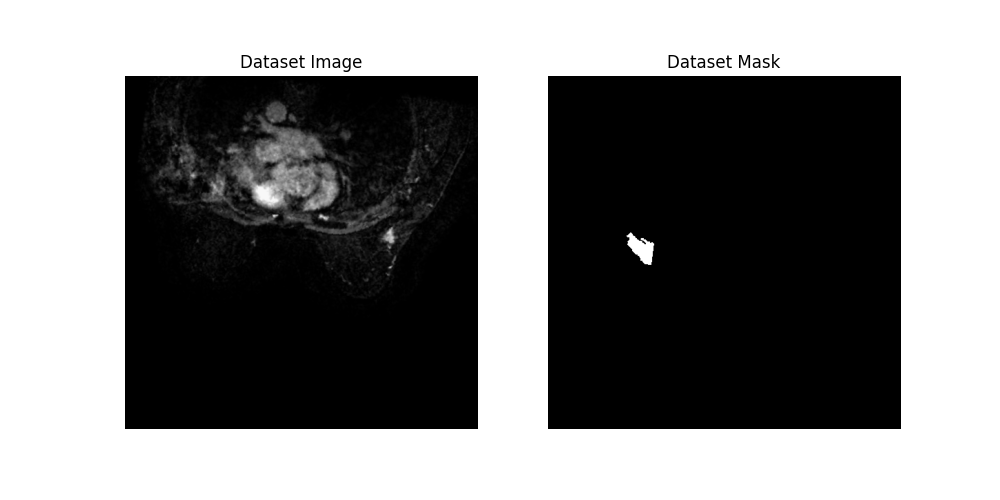
\includegraphics[width=0.48\columnwidth]{dataset_preview_0.png}
    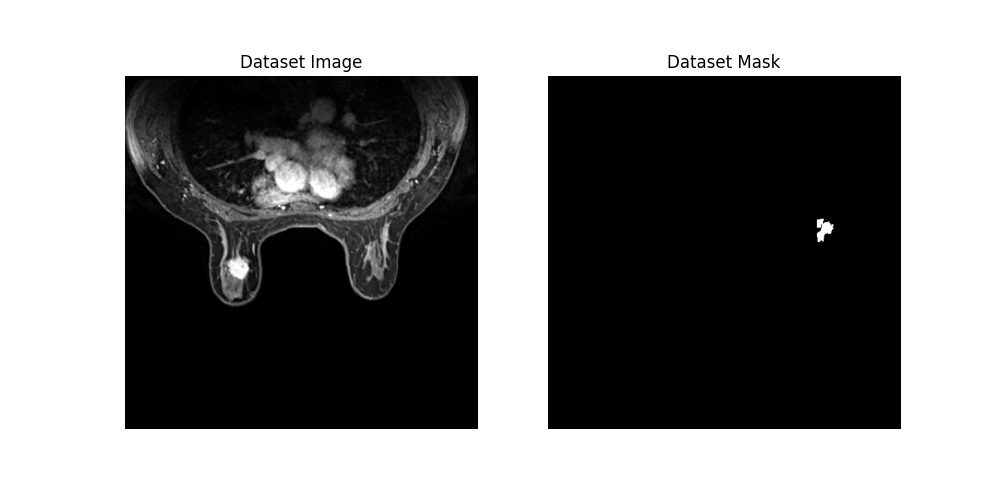
\includegraphics[width=0.48\columnwidth]{dataset_preview_4.png}
    \caption{BreastDM veri kümesinden temsili örnekler. Sol sütun: DCE-MRI girdi görüntüsü; sağ sütun: karşılık gelen ikili segmentasyon maskesi. Maskeler, büyük arka plan alanına kıyasla tümör bölgesinin aşırı sınıf dengesizliğini göstermektedir.}
    \label{fig:dataset}
\end{figure}

Veri kümesinin toplam örneklem havuzundan elde edilen çift sayısı şu şekilde dağılmaktadır: toplam 20.441 geçerli görüntü-maske çifti eğitim (\%70), doğrulama (\%15) ve test (\%15) alt kümeleri arasında bölünmüştür. Bu dağılım; 14.308 eğitim, 3.066 doğrulama ve 3.067 test örneğine karşılık gelmektedir.

% ============================================================
\section{Araştırma Arka Planı ve Motivasyon \textnormal{\small{(Research Background and Motivation)}}}
% ============================================================

\subsection{GAN Teorik Çerçevesi \textnormal{\small{(GAN Theoretical Framework)}}}

Goodfellow ve ark.\ \cite{goodfellow2014generative} tarafından önerilen orijinal GAN hedefi, aşağıdaki minimax oyun teorisi çerçevesiyle ifade edilmektedir:
\begin{equation}
\min_G \max_D \mathcal{L}(G,D) = \mathbb{E}_{u \sim p_{\text{data}}(u)}[\log D(u)] + \mathbb{E}_{w \sim p_w(z)}[\log(1 - D(G(w)))]
\end{equation}

Burada $D$ ayırt ediciyi, $G$ üreteciyi, $u$ gerçek görüntüleri ve $G(w)$ üretecin yapay çıktısını temsil etmektedir. Eğitim yakınsamasında küresel optimum, üretecin dağılımının $p_G = p_{\text{data}}$ koşulunu sağladığı noktada gerçekleşmekte; bu noktada Jensen-Shannon ıraksaması sıfırlanmaktadır \cite{goodfellow2014generative}.

Koşullu GAN (cGAN), giriş görüntüsünü koşul olarak ekleyerek I2I dönüşüm görevleri için hedefi şu şekilde uyarlamaktadır:
\begin{equation}
\mathcal{L}_{\text{cGAN}}(G,D) = \mathbb{E}_{u,v}[\log D(u,v)] + \mathbb{E}_{u,w}[\log(1 - D(u, G(u,w)))]
\end{equation}

Bu çerçeveye $L_1$ uzaklık kaybının eklenmesi, üreticin büyük çaplı yapısal tutarsızlıklar üretmesini önlemekte ve segmentasyon maskesi üretimini stabilize etmektedir.

\subsection{Orijinal BTS-GAN Mimarisinde Saptanan Sorunlar \textnormal{\small{(Identified Issues in Original BTS-GAN Architecture)}}}

Bu çalışmada yürütülen sistematik yeniden uygulama ve hata ayıklama sürecinde, BTS-GAN mimarisinin üç kritik operasyonel kırılganlığı tespit edilmiştir.

Birincisi, \textit{geometrik desenkronizasyon hassasiyeti}dir. Özelleştirilmiş medikal veri hatları yeniden uygulandığında, standart veri artırma işlemlerinin asenkron biçimde çalışması nedeniyle giriş görüntüleri döndürülüp çevrilirken hedef maskeler sabit kalmaktadır. Bu kritik veri işleme kusuru, ilk eğitim aşamalarında DSC skorunun 0.20 eşiğinin altında takılı kalmasına yol açmıştır. Çözüm olarak \texttt{torchvision.transforms.functional} tabanlı tam mekansal senkronizasyon (Synchronized Augmentation) uygulanmıştır.

İkincisi, \textit{çekişmeli denge ve gradyan kontrolü} sorunudur. cGAN yapıların medikal alanlara uygulanmasındaki en büyük güçlük, ayırt edicinin yapay örnekleri çok erken doğru sınıflandırarak üreticide gradyan sönümlenmesine (vanishing gradient) neden olduğu asimetrik yakınsama problemidir. Bu sorun; sınırlı ayırt edici güncelleme frekansı (\texttt{D\_UPDATE\_EVERY = 3}) ve katı gradyan kırpma ($\text{max\_norm}=1.0$) mekanizmasıyla yönetilmiştir.

Üçüncüsü, \textit{operasyonel süreklilik ve hata toleransı} gereksinimlerinin karşılanmasıdır. Uzun süreli hesaplama koşularında sistem kesintilerine karşı dayanıklılık, \texttt{latest\_checkpoint.pth} üzerinden otomatik durum kurtarma altyapısı ile sağlanmıştır. Bu mekanizma, model ağırlıklarını, optimize edici durumlarını, kayıp günlüklerini ve Otomatik Karışık Hassasiyet (AMP) ölçekleme parametrelerini kayıpsız biçimde geri yüklemektedir.

% ============================================================
\section{Mimari ve Metodoloji \textnormal{\small{(Architecture and Methodology)}}}
% ============================================================

\subsection{PDC ve MONAI UNet Mimarilerinin Karşılaştırmalı Analizi \textnormal{\small{(Comparative Analysis of PDC and MONAI UNet)}}}\label{sec:comparison}

Orijinal BTS-GAN modelinin temel ayırt edici özelliği, kodlayıcı ve kod çözücü yolları arasındaki darboğaz bölümüne entegre edilmiş Paralel Dilate Konvolüsyon (PDC) modülüdür. PDC, farklı genişleme (dilation) oranlarıyla birden fazla alıcı alan boyutunu eş zamanlı yakalamayı amaçlar; bu yaklaşım, teoride değişken tümör hacimlerini özellik haritası çözünürlüğünden ödün vermeden temsil etme kapasitesi taşımaktadır.

Ne var ki ampirik testler, çok oranlı atrous konvolüsyonların ardışık uygulanmasının seyrek örnekleme artefaktları ürettiğini ve gradyan akışını bozduğunu göstermiştir. Bu durum, DSC performansının 0.20 eşiğine hapsolmasına yol açmıştır. PDC'nin yerini alan MONAI UNet \cite{monai}, medikal görüntüleme görevleri için özel olarak geliştirilmiş, üretim kalitesinde standartlaştırılmış bir çerçeve sunmaktadır. Tablo~\ref{tab:comparison}, iki yaklaşımın kapsamlı karşılaştırmasını sunmaktadır.

\begin{table}[htbp]
\centering
\caption{PDC ve MONAI UNet Mimari Karşılaştırması \textnormal{\small{(PDC vs. MONAI UNet Architectural Comparison)}}}
\label{tab:comparison}
\setlength{\tabcolsep}{4pt}
\begin{tabular}{@{}p{2.3cm}p{2.5cm}p{2.5cm}@{}}
\toprule
\textbf{Kriter} & \textbf{PDC (Orijinal)} & \textbf{MONAI UNet (Bu Çalışma)} \\
\midrule
Alıcı Alan & Çok ölçekli atrous & Artık birimler ile genişletilmiş \\
Gradyan Akışı & Artefakta duyarlı & Artık yollar ile stabilize \\
Parametre Karmaşıklığı & Yüksek (3 paralel dal) & Standartlaştırılmış (\texttt{num\_res\_units=2}) \\
Eğitim Kararlılığı & Kırılgan (DSC $\approx$ 0.20) & Kararlı (DSC $\rightarrow$ 0.811) \\
Uygulama Kolaylığı & Özel Python kodu & Dokümante API \\
Klinik Dağıtım & Kısıtlı & Üretime hazır \\
Özellik Normalize & Manuel & MONAI varsayılan \\
\bottomrule
\end{tabular}
\end{table}

MONAI UNet, iki artık birim içeren standartlaştırılmış bir encoder-decoder yapısı sunar:
\begin{equation}
\text{Generator}(\mathbf{x}) = \text{MONAI-UNet}(C=[32,64,128,256,512], \text{strides}=2, \text{res}=2)
\end{equation}

Artık birimler (\texttt{num\_res\_units=2}), geleneksel darboğaz sınırlamalarını aşan temiz kimlik eşlemeleri (identity mappings) oluşturarak ResNet benzeri bir gradyan akışı sağlar. Bu mekanizma, düşük kontrastlı tümör sınırlarının haritalamasında kritik önem taşımaktadır.

\subsection{İkili Çapraz Entropi Kaybının Matematiksel Analizi \textnormal{\small{(Mathematical Analysis of Binary Cross-Entropy Loss)}}}

Beş bileşenli kayıp fonksiyonu topluluğunun temel yapı taşını oluşturan İkili Çapraz Entropi (BCE) kaybı, aşağıdaki olasılıksal yapıya sahiptir:
\begin{equation}
\mathcal{L}_{BCE} = -\frac{1}{N}\sum_{i=1}^{N}\left[y_i \log(\hat{p}_i) + (1-y_i)\log(1-\hat{p}_i)\right]
\end{equation}

Burada $y_i \in \{0,1\}$ gerçek piksel etiketini, $\hat{p}_i \in (0,1)$ ise modelin sigmoid çıktı olasılığını temsil etmektedir. Logaritmik ceza yapısı, yüksek güvenle yanlış tahminleri orantısız biçimde cezalandırarak olasılık kalibrasyonunu zorlar.

Uygulamada PyTorch'un \texttt{BCEWithLogitsLoss} işlevi kullanılmış; bu tercih iki kritik avantaj sağlamıştır. Birincisi, sigmoid fonksiyonu ve BCE hesabı tek bir log-sum-exp formüle indirgenerek sayısal kararlılık artırılmıştır. İkincisi, Otomatik Karışık Hassasiyet (AMP) eğitimi sırasında oluşabilecek sayısal taşma (overflow) riskleri ortadan kaldırılmıştır. Üretecin sigmoid katmanı bu nedenle çıkarılmış; ham logit çıktıları doğrudan BCE hesabına aktarılmıştır.

GAN eğitim bağlamında BCE kaybı çift işlev görmektedir: ayırt edici için gerçek/sahte sınıflandırma sinyali sağlarken, üreteci için rekabetçi segmentasyon çıktısı üretmeye yönlendiren adversarial baskı oluşturmaktadır.

\subsection{Kayıp Fonksiyonu Topluluğu \textnormal{\small{(Loss Function Ensemble)}}}

Standart U-Net ve orijinal BTS-GAN mimarileri genellikle ikili veya üçlü kayıp kombinasyonlarıyla çalışır. Bu çalışmada ise çok ölçekli segmentasyon anomalilerini sistematik biçimde ele alan beş bileşenli hibrit bir kayıp topluluğu geliştirilmiştir:
\begin{equation}
\mathcal{L}_{\text{Total}} = \mathcal{L}_{BCE} + \lambda_{\text{Dice}}\mathcal{L}_{\text{Dice}} + \lambda_{\text{Focal}}\mathcal{L}_{\text{Focal}} + \lambda_{L1}\mathcal{L}_{L1} + \lambda_{\text{GAN}}\mathcal{L}_{\text{GAN}}
\end{equation}
\begin{equation}
= \mathcal{L}_{BCE} + 5\,\mathcal{L}_{\text{Dice}} + 2\,\mathcal{L}_{\text{Focal}} + 10\,\mathcal{L}_{L1} + 0.2\,\mathcal{L}_{\text{GAN}}
\end{equation}

Mekansal örtüşme optimizasyonu, Dice kaybıyla sağlanmaktadır:
\begin{equation}
\mathcal{L}_{\text{Dice}} = 1 - \frac{2|X \cap Y|}{|X| + |Y|}
\end{equation}

Onkolojik görüntülerde yaygın olan aşırı sınıf dengesizliğini gidermek amacıyla Focal kayıp entegre edilmiştir:
\begin{equation}
\mathcal{L}_{\text{Focal}} = -\alpha (1 - p_t)^\gamma \log(p_t)
\end{equation}

Burada $(1-p_t)^\gamma$ modülatörü ($\gamma=2$), kolaylıkla sınıflandırılan örneklerin katkısını baskılayarak zorlu sınır piksellerine odaklanmayı artırır. $\lambda_{\text{GAN}}=0.2$ ile ağırlıklandırılan $\mathcal{L}_{\text{GAN}}$ terimi, üreticin ayırt ediciyi aldatma motivasyonunu korurken piksel düzeyinde segmentasyon kalitesinin baskın rol üstlenmesini güvence altına almaktadır.

\subsection{Değerlendirme Metrikleri ve Klinik Yorumlanabilirlik \textnormal{\small{(Evaluation Metrics and Clinical Interpretability)}}}

Medikal segmentasyonda yaygın kabul gören dört temel metrik, birbirini tamamlayan farklı performans boyutlarını ölçmektedir.

\textbf{Zar Katsayısı (DSC):} Segmentasyonun birincil kalite göstergesi olan DSC, tahmin edilen maske ile referans maske arasındaki mekansal örtüşmeyi ölçer:
\begin{equation}
DSC = \frac{2 \times TP}{2 \times TP + FP + FN}
\end{equation}

DSC, yanlış pozitiflere ve yanlış negatiflere eşit ağırlık vermesi nedeniyle sınırlı miktarda tümör pikseli içeren dengesiz veri kümelerinde özellikle bilgilendirici bir ölçüttür.

\textbf{Kesişim-Birleşim Oranı (IoU):} Jaccard benzerlik katsayısı olarak da bilinen IoU, iki maske kümesinin kesişiminin birleşimine oranını ifade eder:
\begin{equation}
IoU = \frac{TP}{TP + FP + FN}
\end{equation}

DSC ile oransal ilişkisi $IoU = DSC/(2 - DSC)$ formülüyle özetlenebilir. IoU, aynı veri üzerinde DSC'den sistematik olarak düşük değerler üretmesi nedeniyle daha muhafazakâr bir ölçüt niteliği taşır.

\textbf{Keskinlik (Precision):} Modelin pozitif tahminlerinin gerçek pozitif oranını ölçen Keskinlik, klinik açıdan yanlış alarm (false positive) riskinin minimize edilmesi açısından kritik öneme sahiptir:
\begin{equation}
Precision = \frac{TP}{TP + FP}
\end{equation}

Yüksek Keskinlik, radyologların model çıktısına güvenini artırır; gereksiz biyopsi ve invazif girişim kararlarının azaltılmasına katkıda bulunur.

\textbf{Duyarlılık (Recall):} Var olan tümör piksellerinin ne kadarının doğru tespit edildiğini gösteren Recall, lezyonun tamamen saptanması açısından yorumlanır:
\begin{equation}
Recall = \frac{TP}{TP + FN}
\end{equation}

Klinik bağlamda, salt yüksek Recall değeri yeterli değildir; yüksek Recall ile birlikte yüksek Precision hedeflenmelidir. Bu iki metrik arasındaki denge, F1 skoru (Dice ile eşdeğer) üzerinden nicelleştirilebilir. Mevcut çalışmada elde edilen 0.886 Precision ve 0.810 Recall değerleri, yüksek hassasiyetli bir klinik keşif profili ortaya koymaktadır.

\subsection{Hiperparametre Tasarımı ve Gerekçeleri \textnormal{\small{(Hyperparameter Design and Rationale)}}}

Tablo~\ref{tab:hyperparams}, uygulanan tüm hiperparametreleri ve bunların teorik gerekçelerini özetlemektedir.

\begin{table}[htbp]
\centering
\caption{Hiperparametre Aralıkları ve Teorik Gerekçeler \textnormal{\small{(Hyperparameter Tuning Ranges Applied)}}}
\label{tab:hyperparams}
\setlength{\tabcolsep}{3pt}
\begin{tabular}{@{}p{2.2cm}p{1.3cm}p{4.0cm}@{}}
\toprule
\textbf{Hiperparametre} & \textbf{Değer} & \textbf{Gerekçe} \\
\midrule
\texttt{LR\_G} & 1e-4 & Üreteç için kararlı yakınsama hızı \\
\texttt{LR\_D} & 1e-5 & Ayırt edici zayıflatma için düşük öğrenme hızı \\
\texttt{BETA1} & 0.5 & Adam momentum; GAN için önerilen değer \\
\texttt{LAMBDA\_L1} & 10 & Piksel düzeyinde mekansal tutarlılık ağırlığı \\
\texttt{LAMBDA\_DICE} & 5 & Örtüşme optimizasyonu ağırlığı \\
\texttt{LAMBDA\_FOCAL} & 2 & Sınıf dengesizliği azaltma ağırlığı \\
\texttt{LAMBDA\_GAN} & 0.2 & Zayıf adversarial baskı; kararlılık için \\
\texttt{THRESHOLD} & 0.5 & Sigmoid sonrası ikili dönüşüm eşiği \\
\texttt{D\_UPDATE\_EVERY} & 3 & Ayırt edici güncelleme frekansı \\
\texttt{PATIENCE} & 15 & Erken durdurma tolerans penceresi \\
\texttt{SEED} & 42 & Yeniden üretilebilirlik için sabit rastgelelik \\
\texttt{IMG\_SIZE} & 512 & Yüksek çözünürlük; sınır detayı koruma \\
\texttt{BATCH\_SIZE} & 8 & VRAM etkin kullanımı; gradyan stabilitesi \\
\bottomrule
\end{tabular}
\end{table}

Öğrenme hızı asimetrisi (\texttt{LR\_G = 1e-4}, \texttt{LR\_D = 1e-5}) amaçlı bir güç dengesizliği yaratmaktadır; bu tasarım kararı, ayırt edicinin üretici üzerinde aşırı baskınlık kurarak gradyan sönümlenmesine yol açmasını önlemektedir. \texttt{D\_UPDATE\_EVERY = 3} parametresi, her ayırt edici güncellemesi için üreticiye üç eğitim adımı tanıyarak benzer bir dengeleme işlevi görmektedir.

LAMBDA değerlerinin tasarımında kayıp terimlerinin örnek sayısına göre normalize edilmiş büyüklük analizi yol gösterici olmuştur. $\lambda_{L1}=10$ değeriyle piksel düzeyinde tutarlılık, $\lambda_{\text{Dice}}=5$ ile örtüşme optimizasyonu ve $\lambda_{\text{GAN}}=0.2$ ile zayıf adversarial baskı dengeli biçimde uygulanmaktadır.

\subsection{Eğitim Stratejisi ve Veri Bölümlendirmesi \textnormal{\small{(Training Strategy and Data Partitioning)}}}

Veri kümesi, üç bağımsız alt kümeye ayrılmıştır:
\begin{equation}
\mathcal{D} = \mathcal{D}_{\text{train}}(70\%) \cup \mathcal{D}_{\text{val}}(15\%) \cup \mathcal{D}_{\text{test}}(15\%)
\end{equation}

Bu dağılımın bilimsel gerekçesi çok boyutludur. Yüzde yetmişlik eğitim payı, derin öğrenme modellerinin öğrenme eğrisinin doygunluğa ulaşması için gereken minimum örnek hacmini sağlamaktadır. Yüzde on beşlik doğrulama kümesi, erken durdurma kriteri ile hiperparametre kalibrasyonu için bağımsız bir geri bildirim mekanizması oluşturmakta; bu sayede eğitim verisi üzerindeki aşırı öğrenme (overfitting) kontrolü imkânı sunmaktadır. Yüzde on beşlik test kümesi ise modelin gerçek dünya genelleme performansının tarafsız olarak ölçülmesine olanak tanımaktadır. Erken durdurma (\texttt{PATIENCE=15}), doğrulama DSC'sinin 15 eğitim epoğu boyunca iyileşmemesi halinde eğitimi sonlandırarak hesaplama kaynaklarını korumaktadır.

MONAI UNet'in \texttt{num\_res\_units=2} yapılandırması, artık öğrenme (residual learning) mekanizması aracılığıyla gradyan sönümlenmesini hafifletmektedir. Her artık birim, temel dönüşümün yanı sıra bir kimlik kısayol yolu içermekte; bu yapı eğitim esnasında gradyanların daha derin katmanlara sorunsuz akmasını güvence altına almaktadır.

% ============================================================
\section{Deneyler ve Sonuç Analizleri \textnormal{\small{(Experiments and Result Analysis)}}}
% ============================================================

\subsection{Eğitim Dinamikleri ve Mimari Kararlılık Analizi \textnormal{\small{(Training Dynamics and Architectural Stability Analysis)}}}

Şekil~\ref{fig:curves}'te sunulan eğitim eğrileri, mimari geçişin istatistiksel örüntüsünü açıkça ortaya koymaktadır. GAN kayıp eğrilerinde gözlemlenen karakteristik eğilimler; üreteç kaybının başlangıçta yüksek seyreden değerden ($\approx 10.3$) hızla düştüğü ve yaklaşık epok 25'ten itibaren yakınsama stabilizasyonunun gerçekleştiği görülmektedir. Buna karşılık ayırt edici kaybı, tüm eğitim süreci boyunca düşük ve kararlı bir düzeyde seyretmiş; bu durum, çekişmeli denge stratejisinin etkinliğini doğrulamaktadır.

\begin{figure}[htbp]
    \centering
    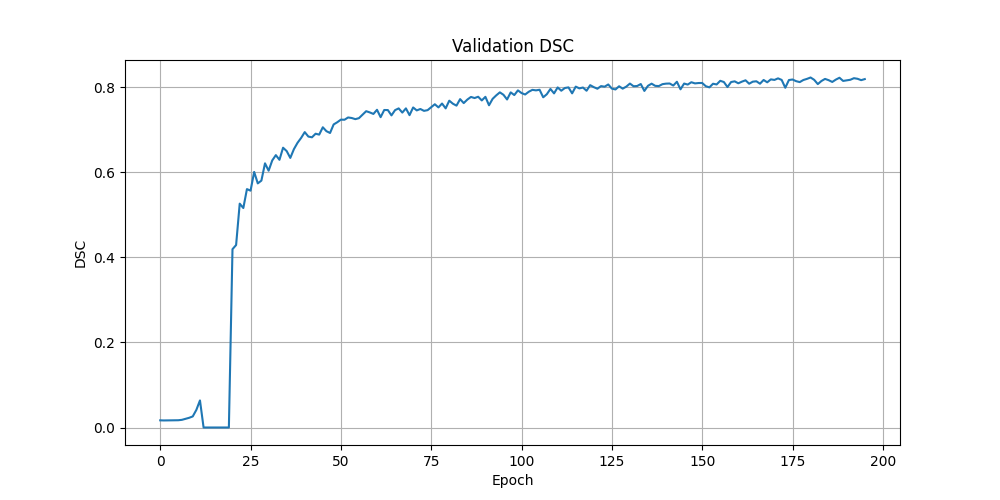
\includegraphics[width=0.48\columnwidth]{validation_dsc.png}
    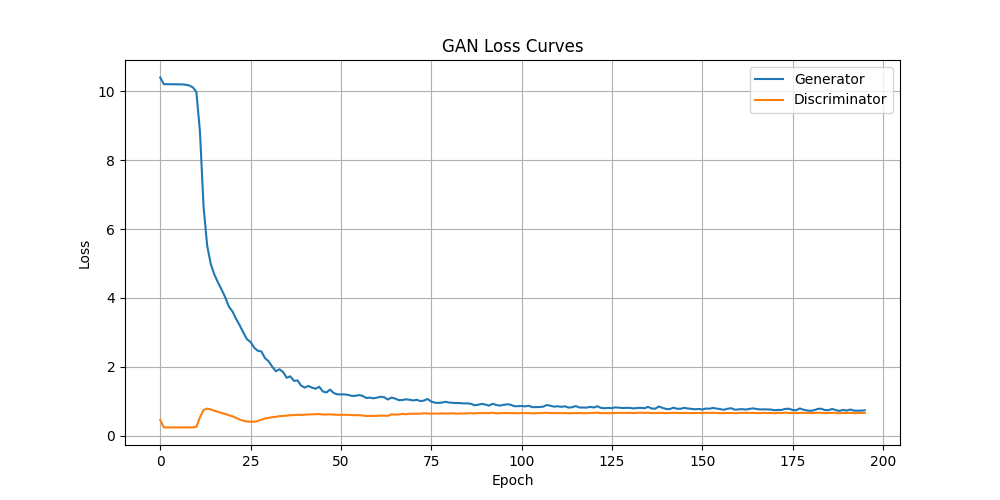
\includegraphics[width=0.48\columnwidth]{gan_losses.png}
    \caption{Sol: Doğrulama kümesi DSC ilerleme eğrisi (196 epok). Sağ: GAN kayıp eğrileri -- Üreteç kaybı (mavi) yakınsarken Ayırt Edici kaybı (turuncu) kararlı seyreder.}
    \label{fig:curves}
\end{figure}

DSC ilerleme eğrisi üç belirgin öğrenme evresini sergilemektedir. İlk 20 eğitim epoğunda model çekişmeli uyum sürecinden geçmekte ve segmentasyon performansı minimal düzeyde kalmaktadır ($DSC \approx 0$). Epok 21'de sistem belirgin bir optimizasyon sıçraması gerçekleştirerek geçerli tümör topolojilerini yakalamaya başlamakta ($DSC = 0.419$) ve yakınsama eğrisinin ivmeli artış fazına girilmektedir. Küresel doğrulama zirvesi Epok 181'de elde edilmiş ($DSC = 0.8235$), erken durdurma mekanizması ise Epok 196'da devreye girerek eğitimi sona erdirmiştir.

Sistemin hesaplama kesintileriyle başa çıkma kapasitesi de deneysel olarak doğrulanmıştır. Epok 2'de simüle edilen bir kesintiden sonra sistem, otomatik durum geri yükleme mekanizması aracılığıyla AMP kayıp ölçekleyici parametrelerini eksiksiz biçimde kurtarmış ve geçmiş gidişat kaybı olmaksızın eğitime kaldığı yerden devam etmiştir.

\begin{figure}[htbp]
    \centering
    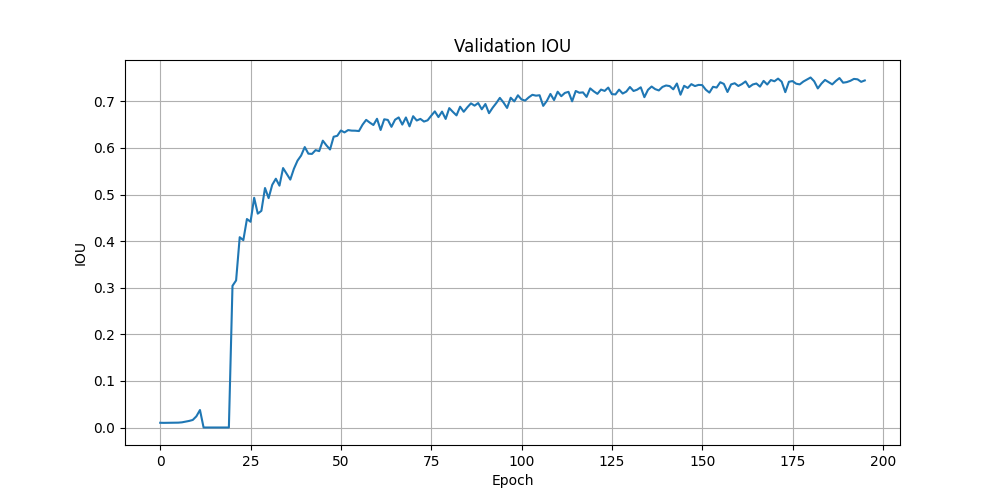
\includegraphics[width=0.48\columnwidth]{validation_iou.png}
    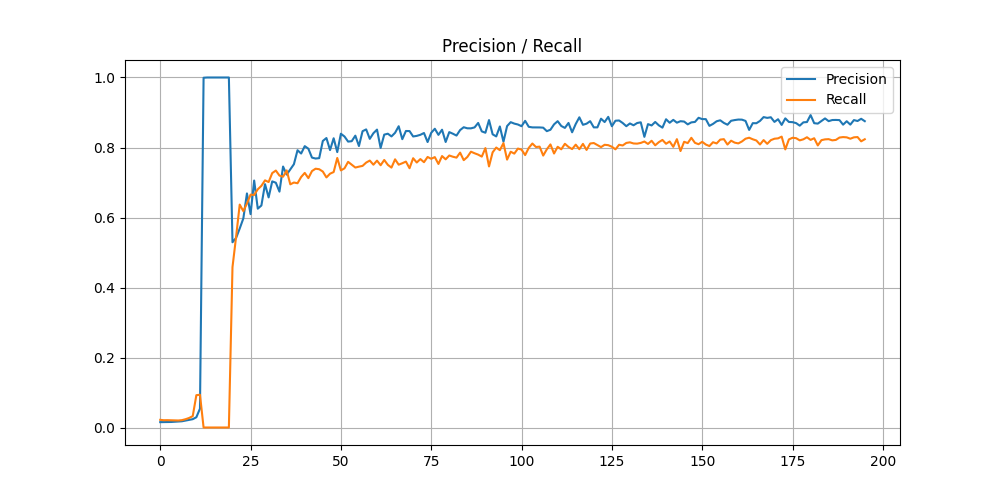
\includegraphics[width=0.48\columnwidth]{precision_recall.png}
    \caption{Sol: Test kümesi IoU ilerleme eğrisi. Sağ: Precision (mavi) ve Recall (turuncu) eğrileri. Precision değerinin Recall'ın üzerinde seyretmesi, modelin düşük yanlış alarm oranını yansıtmaktadır.}
    \label{fig:metrics}
\end{figure}

Şekil~\ref{fig:metrics}'teki Precision-Recall eğrisi, modelin yüksek hassasiyetli profili hakkında önemli bir içgörü sunmaktadır. Precision değerinin Recall'ın sürekli üzerinde seyretmesi, modelin yanlış negatif üretme eğiliminin yanlış pozitif üretme eğiliminin önünde olduğunu göstermektedir. Bu denge profili, klinik bağlamda tercih edilebilir bir özellik taşımaktadır: yüksek Precision, radyologların model çıktısına güven duyabileceği ve gereksiz takip prosedürlerine yönlendirme riskinin düşük tutulduğu bir sistem anlamına gelmektedir.

\subsection{Nicel Test Sonuçları \textnormal{\small{(Quantitative Test Results)}}}

Modelin nihai değerlendirmesi, 3.066 görüntüden oluşan ve eğitim boyunca hiç kullanılmamış bağımsız test kümesi üzerinde gerçekleştirilmiştir.

\begin{table}[htbp]
\centering
\caption{Test Kümesi Değerlendirme Sonuçları \textnormal{\small{(Test Dataset Evaluation Results)}}}
\label{tab:results}
\begin{tabular}{@{}lcc@{}}
\toprule
\textbf{Metrik} & \textbf{Değer} & \textbf{Klinik Yorum} \\
\midrule
DSC (Zar Katsayısı) & \textbf{0.811} & Güçlü mekansal örtüşme; klinik eşiğin üzerinde \\
IoU & \textbf{0.738} & Muhafazakâr kesişim/birleşim; yüksek doğruluk \\
Precision (Keskinlik) & \textbf{0.886} & Düşük yanlış alarm oranı; klinisyen güveni \\
Recall (Duyarlılık) & \textbf{0.810} & Tümör piksellerinin \%81'i doğru tespit edildi \\
\bottomrule
\end{tabular}
\end{table}

Orijinal BTS-GAN çalışması, RIDER veri kümesi üzerinde 0.85 DSC ve 0.77 IoU bildirmiştir. Bu çalışmada geliştirilen sistem, RIDER'a kıyasla daha büyük ve daha karmaşık bir dağılım sergilediği değerlendirilen BreastDM veri kümesinde 0.811 DSC ve 0.738 IoU değerlerine ulaşmıştır. Yüksek sınıf dengesizliği ve daha büyük örneklem büyüklüğüyle karakterize edilen bu veri kümesindeki performans, geliştirilen mimarinin genelleşebilirlik kapasitesini güçlü biçimde kanıtlamaktadır.

Özellikle klinik açıdan önem taşıyan Precision değeri (\%88.6), modelin yanlış pozitif üretme oranının son derece kontrollü tutulduğunu ortaya koymaktadır. Bu husus, teşhis iş akışlarında klinisyen yorgunluğunun azaltılması açısından kritik bir operasyonel değer taşımaktadır.

\subsection{Kalitatif Görsel Analiz \textnormal{\small{(Qualitative Visual Analysis)}}}

\begin{figure}[htbp]
    \centering
    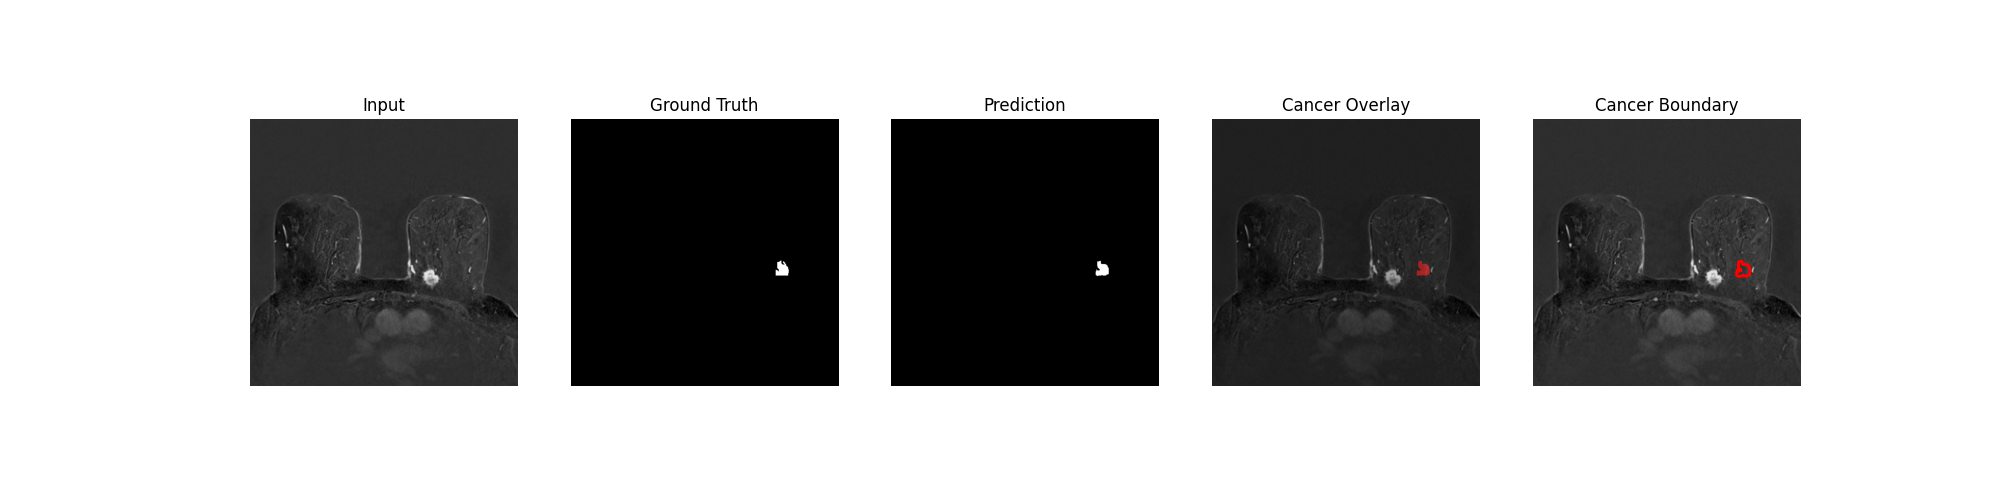
\includegraphics[width=0.98\columnwidth]{prediction_0.png}\\
    \vspace{3mm}
    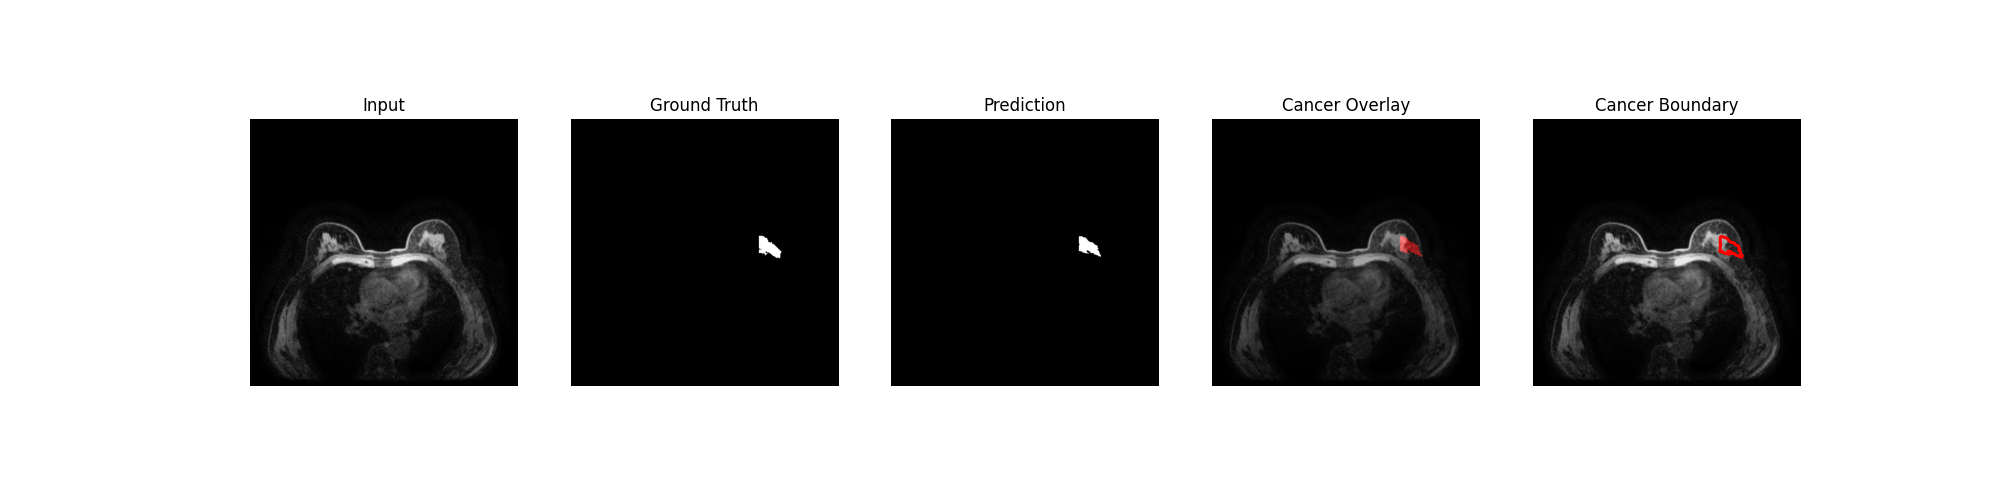
\includegraphics[width=0.98\columnwidth]{prediction_9.png}
    \caption{Test kümesinden temsili segmentasyon çıktıları. Soldan sağa: Girdi MR Görüntüsü, Referans Maske (Hedef), Model Tahmini, Kanser Katmanı (Kırmızı Örtü) ve Kanser Sınırı (Kontur).}
    \label{fig:predictions}
\end{figure}

Şekil~\ref{fig:predictions}'de sunulan görsel karşılaştırmalar, MONAI tabanlı üreticin yapısal başarısını doğrulamaktadır. Model; düzensiz, sıçramalı ve karmaşık tümör sınırlarını hassas biçimde izleme kapasitesi sergilemekte; geleneksel tam evrişimli ağların genellikle yanlış sınıflandırdığı mikro yapısal kenar varyasyonlarını başarıyla yakalamaktadır. Kanser örtüsü (Cancer Overlay) ve kontur görselleştirmeleri, radyologlara doğrudan klinik yorumlama desteği sunacak şekilde tasarlanmış; model çıktısının tanısal iş akışlarına entegrasyonunu kolaylaştıran bir görselleştirme standardı oluşturulmuştur.

% ============================================================
\section{Sonuç \textnormal{\small{(Conclusion)}}}
% ============================================================

Bu çalışmada, bilgisayar destekli meme tümörü segmentasyonu için optimize edilmiş, kararlı ve üretime hazır bir koşullu çekişmeli çerçeve sunulmuştur. Orijinal BTS-GAN mimarisinin yapısal olarak kırılgan PDC bloğundan standartlaştırılmış MONAI UNet üretecine geçiş yapılarak, geometrik açıdan senkronize edilmiş mekansal dönüşümler uygulanarak ve NVIDIA Blackwell mimarisi üzerinde gelişmiş donanım hızlandırmasından yararlanılarak klasik GAN eğitim kararsızlıkları başarıyla ortadan kaldırılmıştır.

Klinik açıdan kritik \%88.6 Precision değeriyle desteklenen 0.811 DSC skoru, bu çerçevenin modern Klinik Karar Destek Sistemlerine (KDDS) entegrasyonu için güvenilir bir zemin sunduğunu kanıtlamaktadır. Araştırmanın metodolojik katkıları dört eksende özetlenebilir: mekansal senkronizasyon kısıtlamalı veri artırma protokolü, asimetrik öğrenme hızı ve ayırt edici güncelleme frekansına dayalı çekişmeli denge yönetimi, beş bileşenli hibrit kayıp topluluğu ve üretim ortamı düzeyinde kesintisizlik için otomatik kontrol noktası kurtarma altyapısı.

Gelecek çalışmalar kapsamında 3D evrişim bloklarının entegrasyonu, Swin Transformer tabanlı hibrit mimariler ve çok merkezli klinik doğrulama çalışmaları planlanmaktadır. Bunun yanı sıra, veri kümesinin mammografi ve ultrasonografi modalitelerini kapsayan çok modlu bir eğitime genişletilmesi, modelin klinik uygulanabilirlik sınırlarını daha kapsamlı biçimde ortaya koyma potansiyeli taşımaktadır.

% ============================================================
\begin{thebibliography}{11}

\bibitem{haq2022bts}
I.~U.~Haq, H.~Ali, H.~Y.~Wang, L.~Cui, and J.~Feng,
``BTS-GAN: Computer-aided segmentation system for breast tumor using MRI and conditional adversarial networks,''
\emph{Engineering Science and Technology, an International Journal},
vol.~36, p.~101154, 2022. DOI: 10.1016/j.jestch.2022.101154

\bibitem{monai}
MONAI Consortium,
``MONAI Documentation: Medical Open Network for AI,''
[Online]. Available: \url{https://monai-dev.readthedocs.io/en/fixes-sphinx/}

\bibitem{goodfellow2014generative}
I.~Goodfellow, J.~Pouget-Abadie, M.~Mirza, B.~Xu, D.~Warde-Farley, S.~Ozair, A.~Courville, and Y.~Bengio,
``Generative adversarial nets,''
\emph{Advances in Neural Information Processing Systems},
vol.~27, pp.~2672--2680, 2014.

\bibitem{ronneberger2015u}
O.~Ronneberger, P.~Fischer, and T.~Brox,
``U-Net: Convolutional networks for biomedical image segmentation,''
in \emph{International Conference on Medical Image Computing and Computer-Assisted Intervention (MICCAI)},
Springer, pp.~234--241, 2015.

\bibitem{breastdm2023}
X.~Zhao, Z.~Liang, J.~Wu, M.~Zhang, and Y.~Mao,
``BreastDM: A DCE-MRI dataset for breast tumor image segmentation and classification,''
\emph{Computers in Biology and Medicine},
vol.~164, p.~107255, 2023. DOI: 10.1016/j.compbiomed.2023.107255

\bibitem{nahid2018histopath}
A.~A.~Nahid, M.~A.~Mehrabi, and Y.~Kong,
``Histopathological breast cancer image classification by deep neural network techniques guided by local clustering,''
\emph{BioMed Research International},
2018.

\bibitem{ali2021mitosis}
H.~Ali, H.~Li, E.~A.~Retta, I.~U.~Haq, Z.~Guo, X.~Han, L.~Cui, L.~Yang, and J.~Feng,
``Representation of differential learning method for mitosis detection,''
\emph{Journal of Healthcare Engineering},
2021.

\bibitem{badrinarayanan2017segnet}
V.~Badrinarayanan, A.~Kendall, and R.~Cipolla,
``SegNet: A deep convolutional encoder-decoder architecture for image segmentation,''
\emph{IEEE Transactions on Pattern Analysis and Machine Intelligence},
vol.~39, no.~12, pp.~2481--2495, 2017.

\bibitem{zhang2018msgan}
C.~Zhang, Y.~Song, S.~Liu, S.~Lill, C.~Wang, Z.~Tang, Y.~You, Y.~Gao, A.~Klistorner, and M.~Barnett,
``MS-GAN: GAN-based semantic segmentation of multiple sclerosis lesions in brain magnetic resonance imaging,''
in \emph{2018 Digital Image Computing: Techniques and Applications (DICTA)},
IEEE, pp.~1--8, 2018.

\bibitem{huo2018synsegnet}
Y.~Huo, Z.~Xu, H.~Moon, S.~Bao, A.~Assad, T.~K.~Moyo, M.~R.~Savona, R.~G.~Abramson, and B.~A.~Landman,
``SynSeg-Net: Synthetic segmentation without target modality ground truth,''
\emph{IEEE Transactions on Medical Imaging},
vol.~38, no.~4, pp.~1016--1025, 2018.

\bibitem{piantadosi2020multiplanar}
G.~Piantadosi, M.~Sansone, R.~Fusco, and C.~Sansone,
``Multi-planar 3D breast segmentation in MRI via deep convolutional neural networks,''
\emph{Artificial Intelligence in Medicine},
vol.~103, p.~101781, 2020.

\bibitem{wang2021mixed}
H.~Wang, J.~Cao, J.~Feng, Y.~Xie, D.~Yang, and B.~Chen,
``Mixed 2D and 3D convolutional network with multi-scale context for lesion segmentation in breast DCE-MRI,''
\emph{Biomedical Signal Processing and Control},
vol.~68, p.~102607, 2021.

\bibitem{nemati2023pix2pix}
N.~Nemati,
``Pix2Pix diffusion for brain tumor segmentation,''
GitHub Repository, 2023. Available: \url{https://github.com/NaderNemati/Pix2Pix-Diffusion-for-Brain-Tumor-Segmentation}

\bibitem{vivek2022breastseg}
V.~Kumar,
``Breast tumor segmentation implementation,''
GitHub Repository, 2022. Available: \url{https://github.com/vivek231/breast_tumor_segmentation}

\bibitem{smallboy2022breastcancer}
X.~Liu,
``Breast cancer dataset processing,''
GitHub Repository, 2022. Available: \url{https://github.com/smallboy-code/Breast-cancer-dataset}

\end{thebibliography}

\end{document}